\documentclass[../Main.tex]{subfiles}

\begin{document}
\author{Resistivity} %use author for title of lesson
\date{Year 1 Topic 13} %use date to refer to topic in main booklet

\section{Resistivity} %Section is the title of the lesson repeated, ready for the main contents page.

\begin{frame}{Resistance of a wire}
    There are 4 things that affect the resistance of a wire:
    \begin{itemize}
        \item The length of the wire -- m
        \item The cross-sectional area of the wire -- m$^2$
        \item Temperature of the wire
        \item The \emph{resistivity} of the wire -- 
    \end{itemize} \pause
    
    The resistivity is a property of the material of the wire that describes how well it resists current. A metal will have a different resistivity for a different temperature. 
    
    \begin{multicols}{2}
    For an ideal conductor, you would have a lower resistivity. Often this is of the order of $10^{-8}$ with units $\Omega m$, but typical insulators will have a resistivity on the order $10^{10} \Omega m$.
    \columnbreak
    \begin{figure}
        \centering
        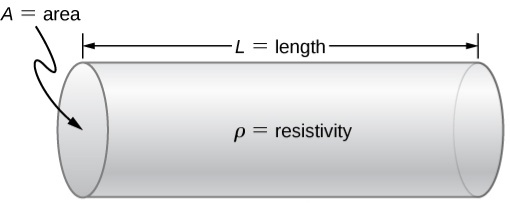
\includegraphics[width=5cm]{Electricity_Images/resistivity.jpg}
    \end{figure}
    \end{multicols}
    \end{frame}

\begin{frame}{Resistance of a wire}
    \begin{figure}
        \centering
        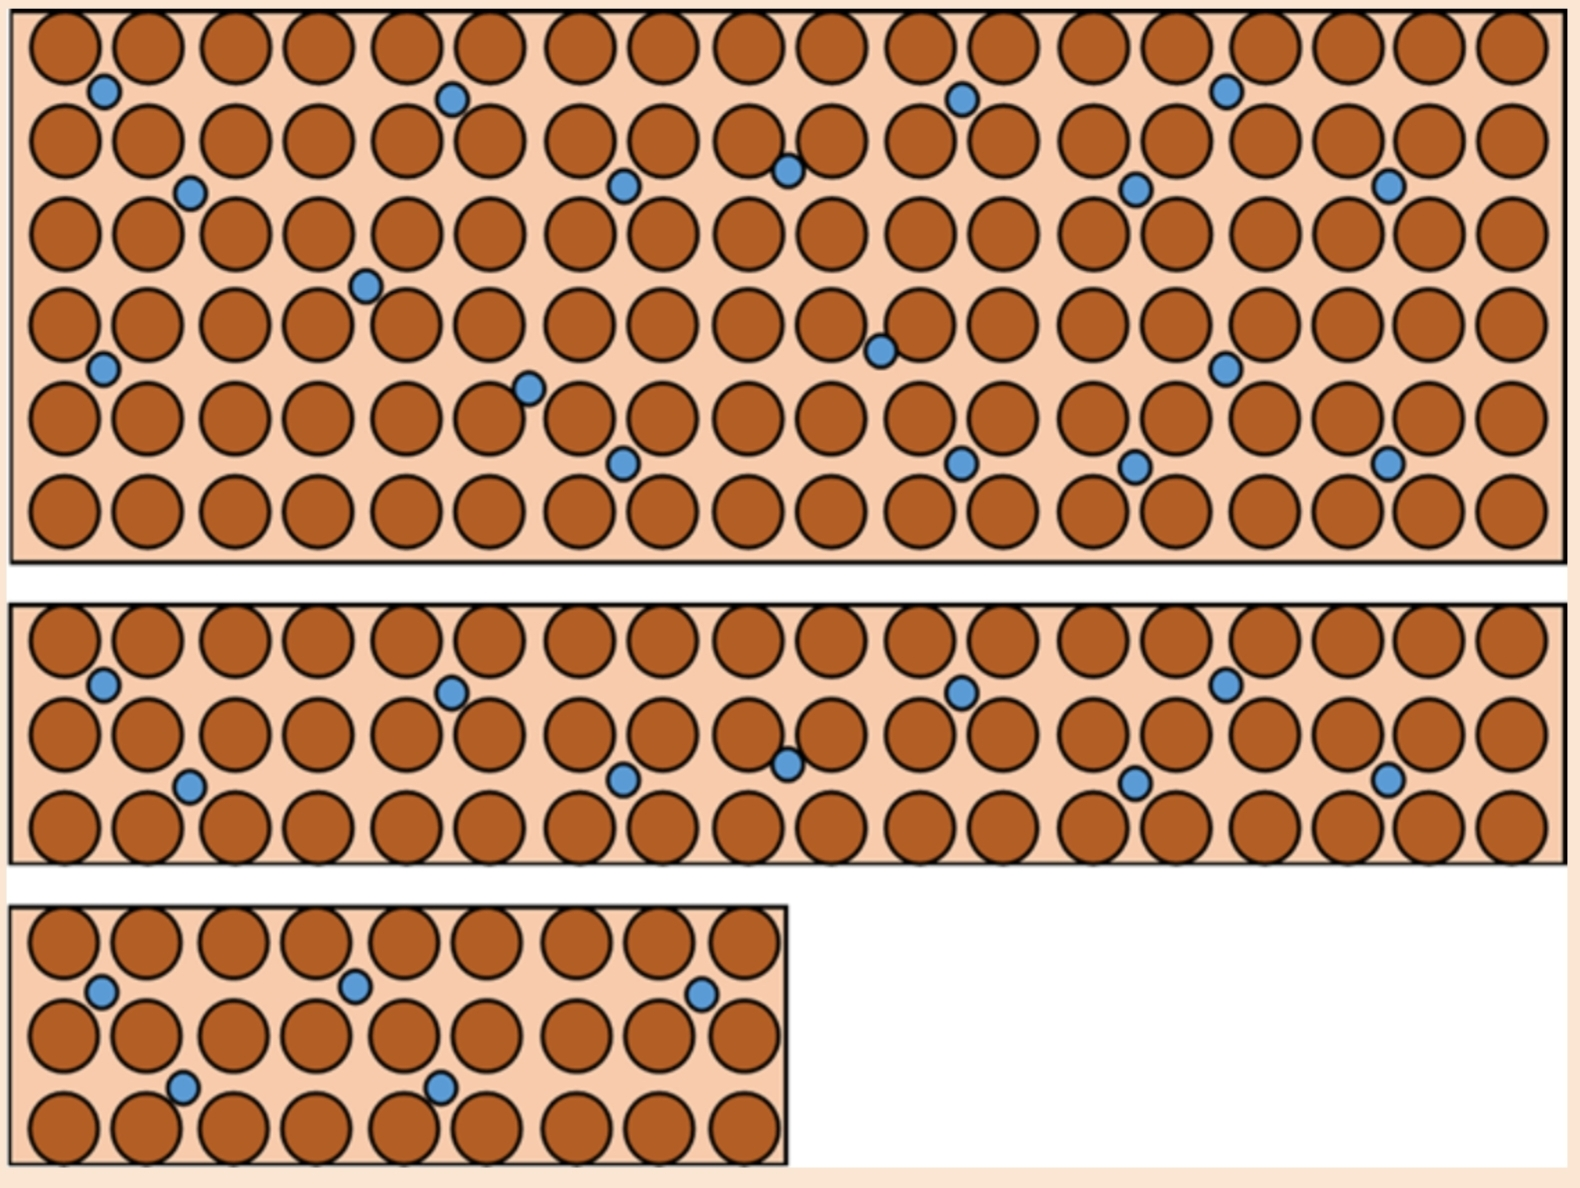
\includegraphics[width=9cm]{Electricity_Images/different_wires.jpg}
    \end{figure} \pause
    The 2nd wire would have the highest resistance.
    
\end{frame}

\begin{frame}{Resistivity}
The equation for resistivity is as follows, and is given on the formula sheet:
    {\huge
    \begin{equation*}
        R =\frac{\rho L}{A} \hspace{1cm} \mbox{units: } [\Omega]=\frac{[\Omega m] [m]}{[m^2]}
    \end{equation*}}
    \pause
    \begin{exampleblock}{Example}
    A circular wire has a diameter of 1mm and a length of 10cm. The resistance is measured to be $2.5\times 10^{-3}\Omega$. Calculate the resistivity of the metal. \pause
    --$1.96\times 10^{-8} \Omega m$
    \end{exampleblock}
    \pause
    \begin{exampleblock}{Example}
    At room temperature a metal has a resistivity of $4.5 \times 10^{–7} \Omega m$. A wire made from this metal has a radius of 0.70 mm. Calculate the resistance of a 2.5 m length of the wire. \pause
    --0.73$\Omega$
    \end{exampleblock}
\end{frame}

\begin{frame}{Resistivity \& temperature}
    Recall our temperature relation from earlier. There's no exact formula for this, but if we were to plot an approximate graph for a typical conducting material we would see: 
    
    \begin{figure}
        \centering
        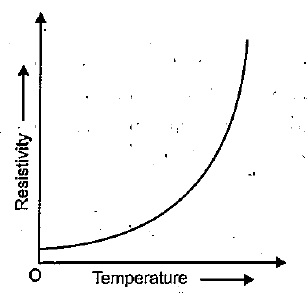
\includegraphics[width=6cm]{Electricity_Images/resistivity_temperature.jpg}
    \end{figure}
\end{frame}

\begin{frame}{Superconductors}
    A superconductor is a conducting material where, below a certain certain temperature -- known as the \emph{critical temperature} -- the resistivity is 0 {\Omega}m.
    
    \begin{figure}
        \centering
        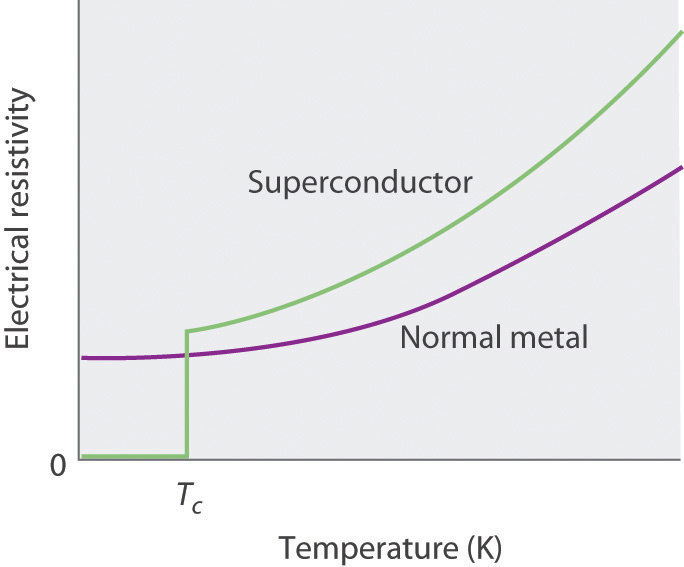
\includegraphics[width=5cm]{Electricity_Images/critical_temp.jpg}
    \end{figure}
    \begin{figure}
        \centering
        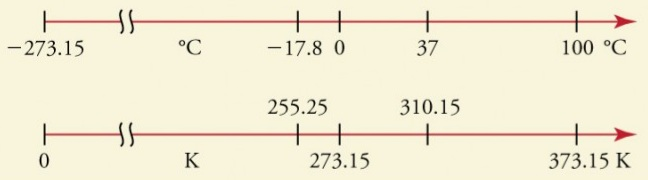
\includegraphics[width=5cm]{Electricity_Images/kelvin_scale.jpg}
    \end{figure}
\end{frame}

\begin{frame}{Conductors}
    \begin{figure}
        \centering
        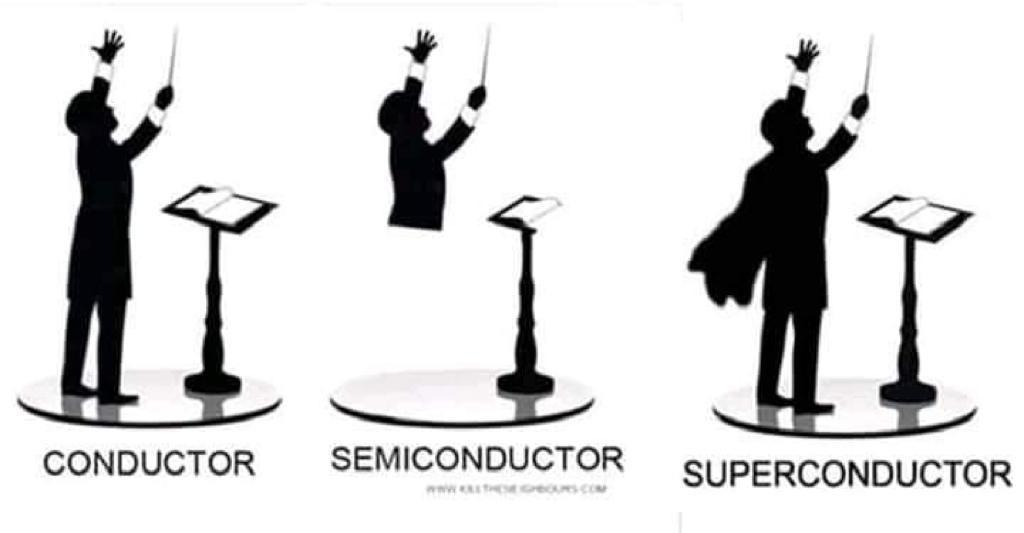
\includegraphics[height=3.5cm]{Electricity_Images/conductors.jpg}
    \end{figure}
    \pause
    \begin{figure}
        \centering
        
\includegraphics[height=3.5cm]{Electricity_Images/floor_is_magnetic_field.jpg}
    \end{figure}
\end{frame}

\begin{frame}{Power loss due to Resistivity}
    Since a wire has a resistance R, with a current `I' there will be a power loss $P=I^2R$. This is not useful if you are trying to deliver power across a country -- for example like the National Grid. 
    \pause
    \newline
    
    So how could we reduce the power loss, if we cannot change the dimensions or material of our cables? \pause
    \newline
    
    \begin{multicols}{2}
    We know that $P\propto I^2$, and $I\propto \frac{1}{V}$ meaning that if we increase the voltage, we will decrease the current. 

    The National Grid transmits power on the order of $10^2$kV, with a very small current, thus reducing the power loss during transmission.
    \newline \newline
    {\tiny *we do not need to know how transformers work, this comes up in 2nd year magnetic fields}
    \columnbreak
    \begin{figure}
        \centering
        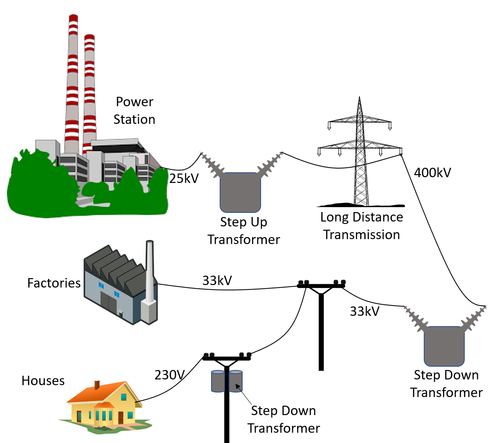
\includegraphics[height=4cm]{Electricity_Images/national_grid.png}
    \end{figure}
\end{multicols}
\end{frame}

\begin{frame}{Superconducting transmission of power}
    If we have a superconductor transmitting power for the national grid or round our homes, we could have a power system that has no waste -- the national grid would be 100\% efficient!
    \pause
    \newline \newline
    Unfortunately, most superconductors have very low critical temperatures and the national grid operates in temperatures up to 300K at the peak of summer. We do not yet have a superconductor that is superconducting at the usual `human' temperatures. \newline \newline
    This is where you guys could come in -- there would be BIG money to the person (or people) who discover a room temperature superconductor! A career in research could take you to fame and fortune.
\end{frame}

\end{document}